% Digital Logic Report Template
% Created: 2020-01-10, John Miller

%==========================================================
%=========== Document Setup  ==============================

% Formatting defined by class file
\documentclass[11pt]{article}

% ---- Document formatting ----
\usepackage[margin=1in]{geometry}	% Narrower margins
\usepackage{booktabs}				% Nice formatting of tables
\usepackage{graphicx}				% Ability to include graphics

%\setlength\parindent{0pt}	% Do not indent first line of paragraphs 
\usepackage[parfill]{parskip}		% Line space b/w paragraphs
%	parfill option prevents last line of pgrph from being fully justified

% Parskip package adds too much space around titles, fix with this
\RequirePackage{titlesec}
\titlespacing\section{0pt}{8pt plus 4pt minus 2pt}{3pt plus 2pt minus 2pt}
\titlespacing\subsection{0pt}{4pt plus 4pt minus 2pt}{-2pt plus 2pt minus 2pt}
\titlespacing\subsubsection{0pt}{2pt plus 4pt minus 2pt}{-6pt plus 2pt minus 2pt}

% ---- Hyperlinks ----
\usepackage[colorlinks=true,urlcolor=blue]{hyperref}	% For URL's. Automatically links internal references.

% ---- Code listings ----
\usepackage{listings} 					% Nice code layout and inclusion
\usepackage[usenames,dvipsnames]{xcolor}	% Colors (needs to be defined before using colors)

% Define custom colors for listings
\definecolor{listinggray}{gray}{0.98}		% Listings background color
\definecolor{rulegray}{gray}{0.7}			% Listings rule/frame color

% Style for Verilog
\lstdefinestyle{Verilog}{
	language=Verilog,					% Verilog
	backgroundcolor=\color{listinggray},	% light gray background
	rulecolor=\color{blue}, 			% blue frame lines
	frame=tb,							% lines above & below
	linewidth=\columnwidth, 			% set line width
	basicstyle=\small\ttfamily,	% basic font style that is used for the code	
	breaklines=true, 					% allow breaking across columns/pages
	tabsize=3,							% set tab size
	commentstyle=\color{gray},	% comments in italic 
	stringstyle=\upshape,				% strings are printed in normal font
	showspaces=false,					% don't underscore spaces
}

% How to use: \Verilog[listing_options]{file}
\newcommand{\Verilog}[2][]{%
	\lstinputlisting[style=Verilog,#1]{#2}
}




%======================================================
%=========== Body  ====================================
\begin{document}

\title{ELC 2137 Lab 10: Lab 10 7-segment Display with Time-Division Multiplexing}
\author{Makenna Meyers}

\maketitle


\section*{Summary}
 This lab incorporates registers and an Arithmetic Logic Unit (ALU) to build a small calculator. The code used can be found in Listings \ref{code:counter}, \ref{code:counter_test}, \ref{code:sseg4_TDM}, \ref{code:sseg4_TDM_test}, and \ref{code:calc_module}. Schematics for the 7-seg driver and calculator modules can be found in Figures \ref{fig:sseg4_TDM_schematic} and \ref{fig:calc_schematic}, respectively. 
 
 \section*{Q/A}
 \begin{enumerate}
 	\item What are the three main "groups" of the RTL definition of sequential logic?
 	
 	state memory, next-state, and output logic
 	
 	\item Include an annotated figure 10.3b below.
 	
 \begin{figure}[ht]\centering
 	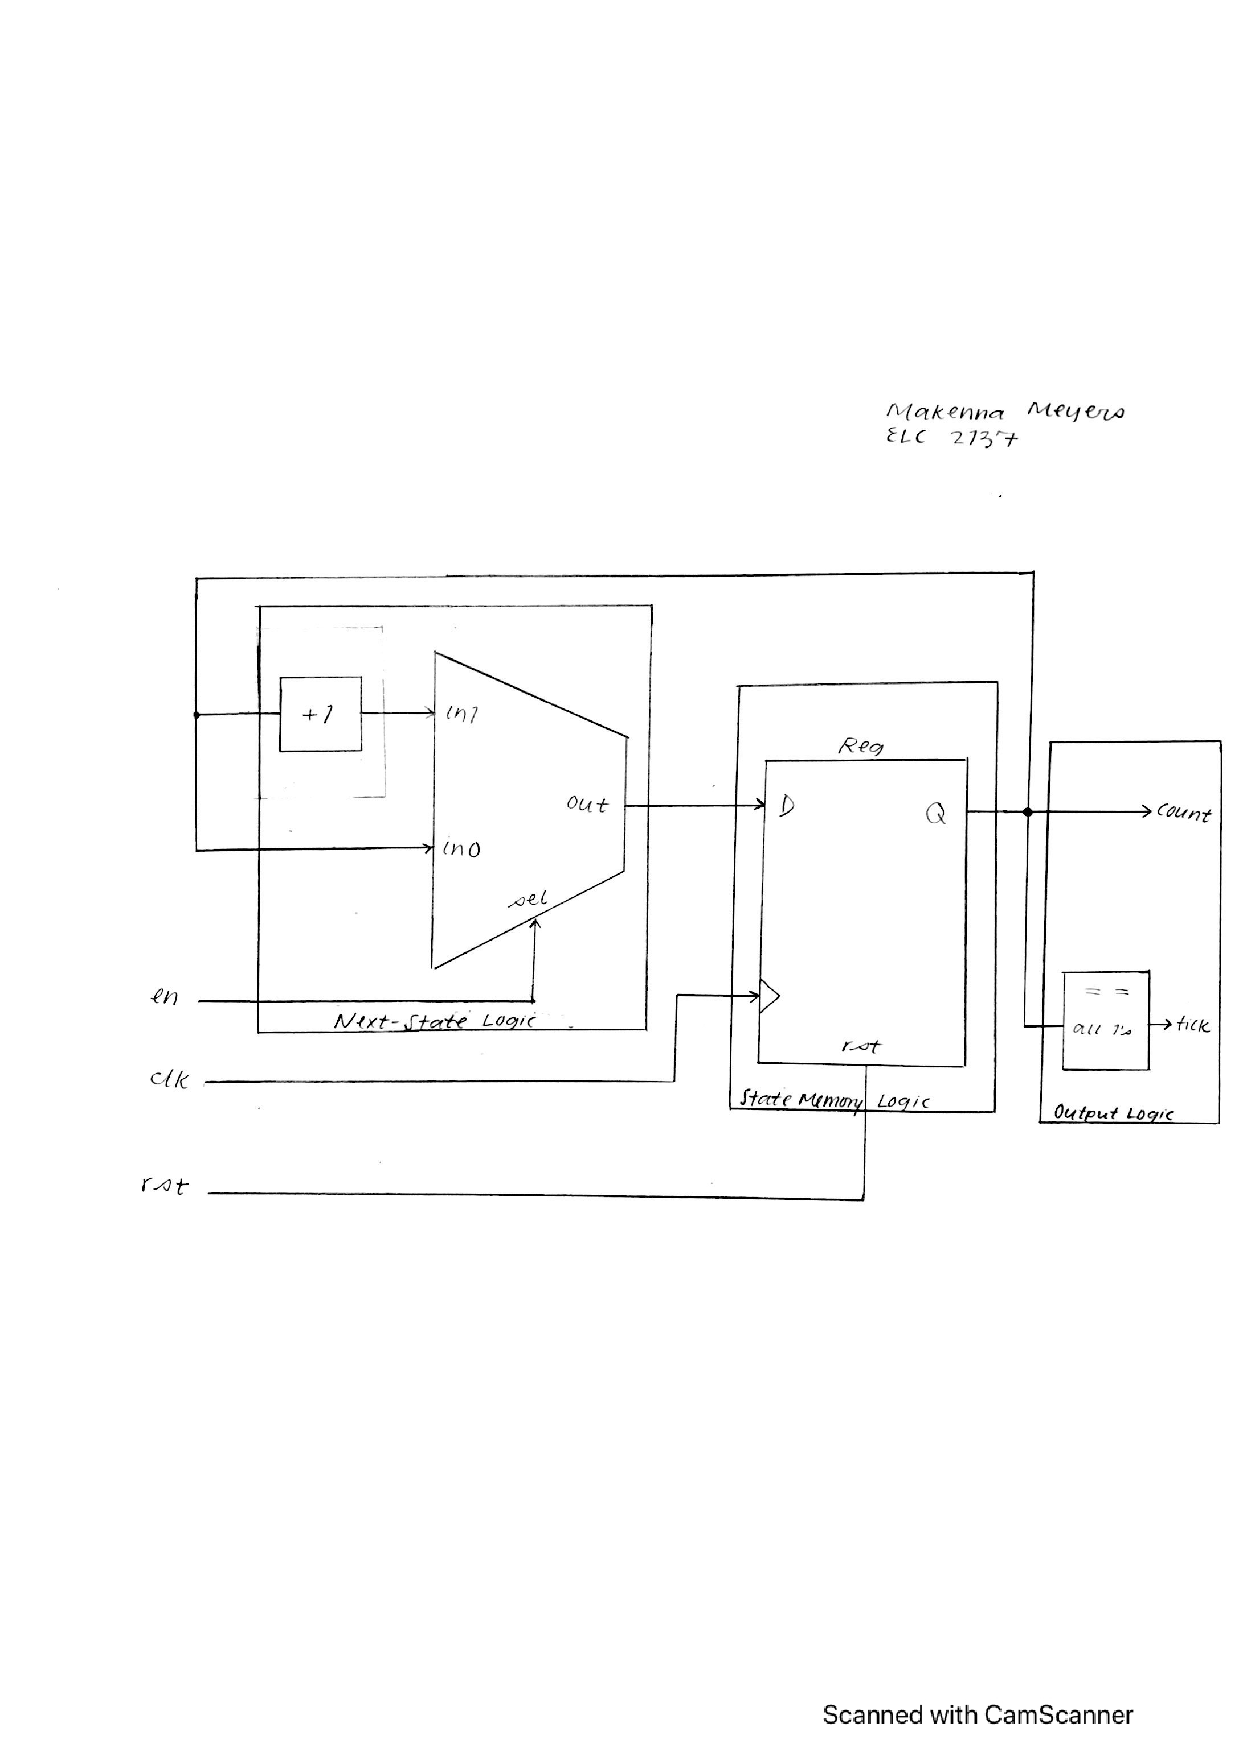
\includegraphics[width=0.8\textwidth,trim=2cm 8cm 0cm 9cm,clip]{annotated_figure}
 	\caption{Annotated Figure 10.3b}
 	\label{fig:annotated_figure}			
 \end{figure}
 \clearpage
 	
 	\item If instead of a counter, you wanted to make a shift register that moved the input bits from right to left (low to high), what would you put on the line $Q_next = /*??*/$?
 	
 	$Q_next = Q_reg-1$
 	
 \end{enumerate}


\section*{Results}

\begin{table*}[ht]\centering
	\caption{\textit{counter} expected results table for time 0 through 45 (ns)}
	\label{ALU:tbl:counter_ERT_1}\medskip
	\begin{tabular}{l|rrrrrrrrr}
		Time (ns): & 0-5 & 5-10 & 10-15 & 15-20 & 20-25 & 25-30 & 30-35 & 35-40 & 40-45 \\
		\midrule
		clk & 0 & 1 & 0 & 1 & 0 & 1 & 0 & 1 & 0 \\
		en  & 1 & 1 & 1 & 1 & 1 & 1 & 1 & 1 & 1 \\
		rst & 1 & 1 & 1 & 1 & 1 & 0 & 1 & 1 & 1 \\
		count & 0 & 0 & 0 & 0 & 0 & 0 & 0 & 0 & 0 \\
		tick & 0 & 0 & 0 & 0 & 0 & 0 & 0 & 0 & 0 \\
		\bottomrule
	\end{tabular}
\end{table*}

\begin{table*}[ht]\centering
	\caption{\textit{counter} expected results table for time 45 through 90 (ns)}
	\label{ALU:tbl:counter_ERT_2}\medskip
	\begin{tabular}{l|rrrrrrrrr}
		Time (ns): & 45-50 & 50-55 & 55-60 & 60-65 & 65-70 & 70-75 & 75-80 & 80-85 & 85-90 \\
		\midrule
		clk & 1 & 0 & 1 & 0 & 1 & 0 & 1 & 0 & 1 \\
		en  & 1 & 0 & 0 & 0 & 0 & 0 & 0 & 1 & 1 \\
		rst & 1 & 0 & 0 & 0 & 0 & 0 & 0 & 0 & 0 \\
		count & 0 & 0 & 0 & 0 & 0 & 0 & 0 & 0 & 0 \\
		tick & 0 & 0 & 0 & 0 & 0 & 0 & 0 & 0 & 0 \\
		\bottomrule
	\end{tabular}
\end{table*}

\begin{table*}[ht]\centering
	\caption{\textit{counter} expected results table for time 90 through 135 (ns)}
	\label{ALU:tbl:counter_ERT_3}\medskip
	\begin{tabular}{l|rrrrrrrrr}
		Time (ns): & 90-95 & 95-100 & 100-105 & 105-110 & 110-115 & 115-120 & 120-125 & 125-130 & 130-135 \\
		\midrule
		clk & 0 & 1 & 0 & 1 & 0 & 1 & 0 & 1 & 0 \\
		en  & 0 & 0 & 1 & 1 & 1 & 1 & 1 & 1 & 1 \\
		rst & 0 & 0 & 0 & 0 & 0 & 0 & 0 & 0 & 0 \\
		count & 0 & 0 & 0 & 1 & 1 & 2 & 2 & 3 & 3 \\
		tick & 0 & 0 & 0 & 0 & 0 & 0 & 0 & 1 & 1 \\
		\bottomrule
	\end{tabular}
\end{table*}

\begin{figure}[ht]\centering
	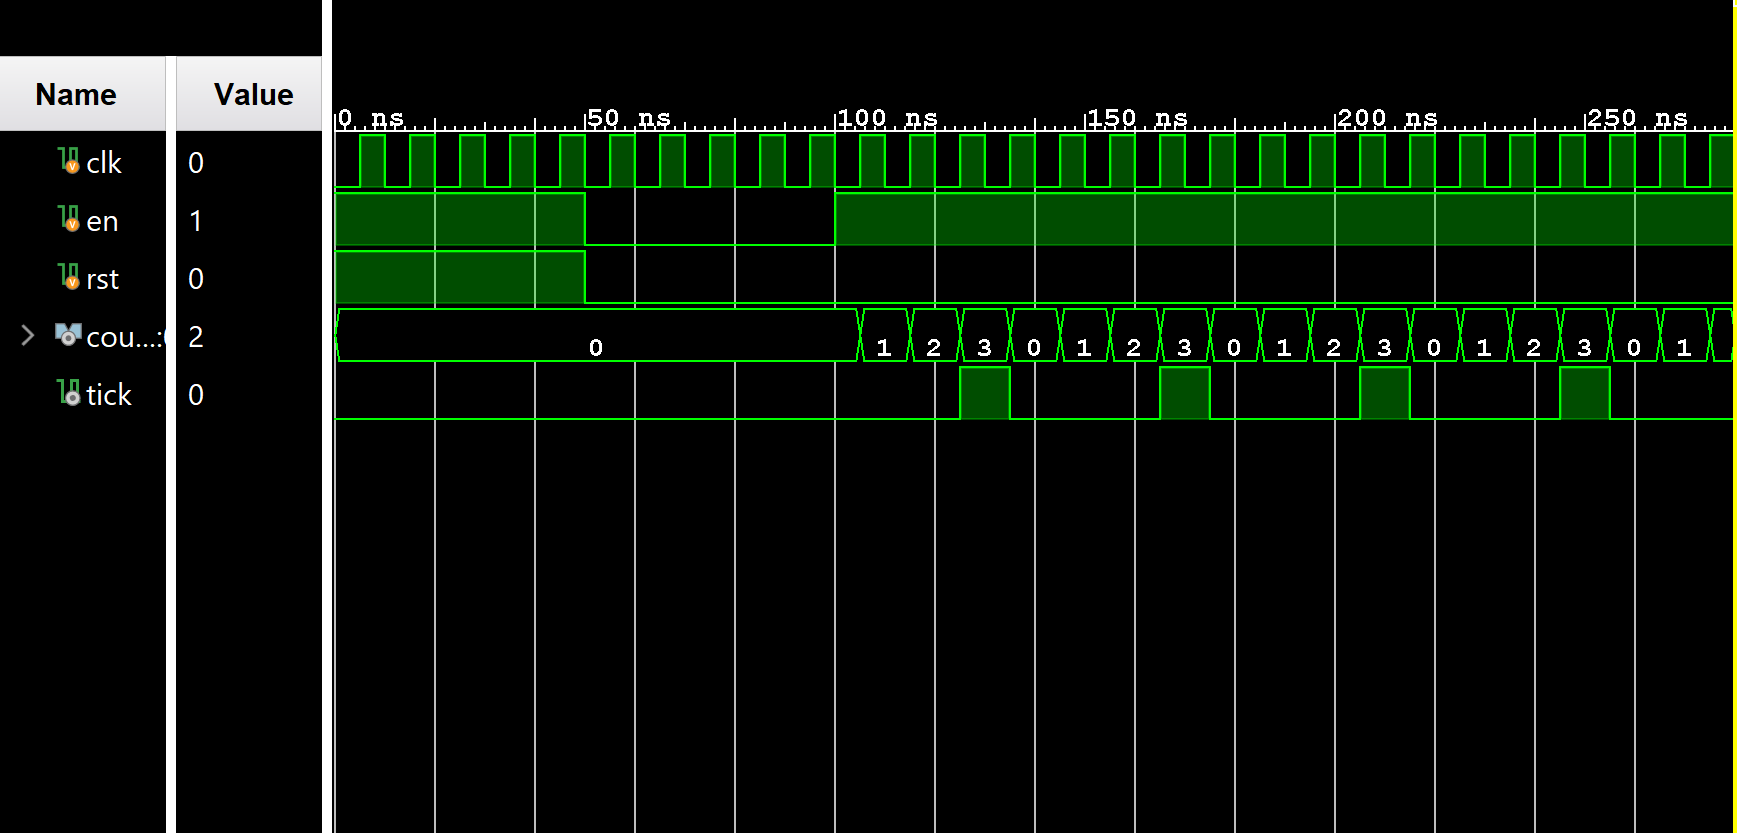
\includegraphics[width=0.8\textwidth,trim=0cm 0cm 0cm 0cm,clip]{counter_test_simwave(1)}
	\caption{Counter Simulation Waveform}
	\label{fig:counter_simwave}			
\end{figure}
\clearpage

\begin{figure}[ht]\centering
	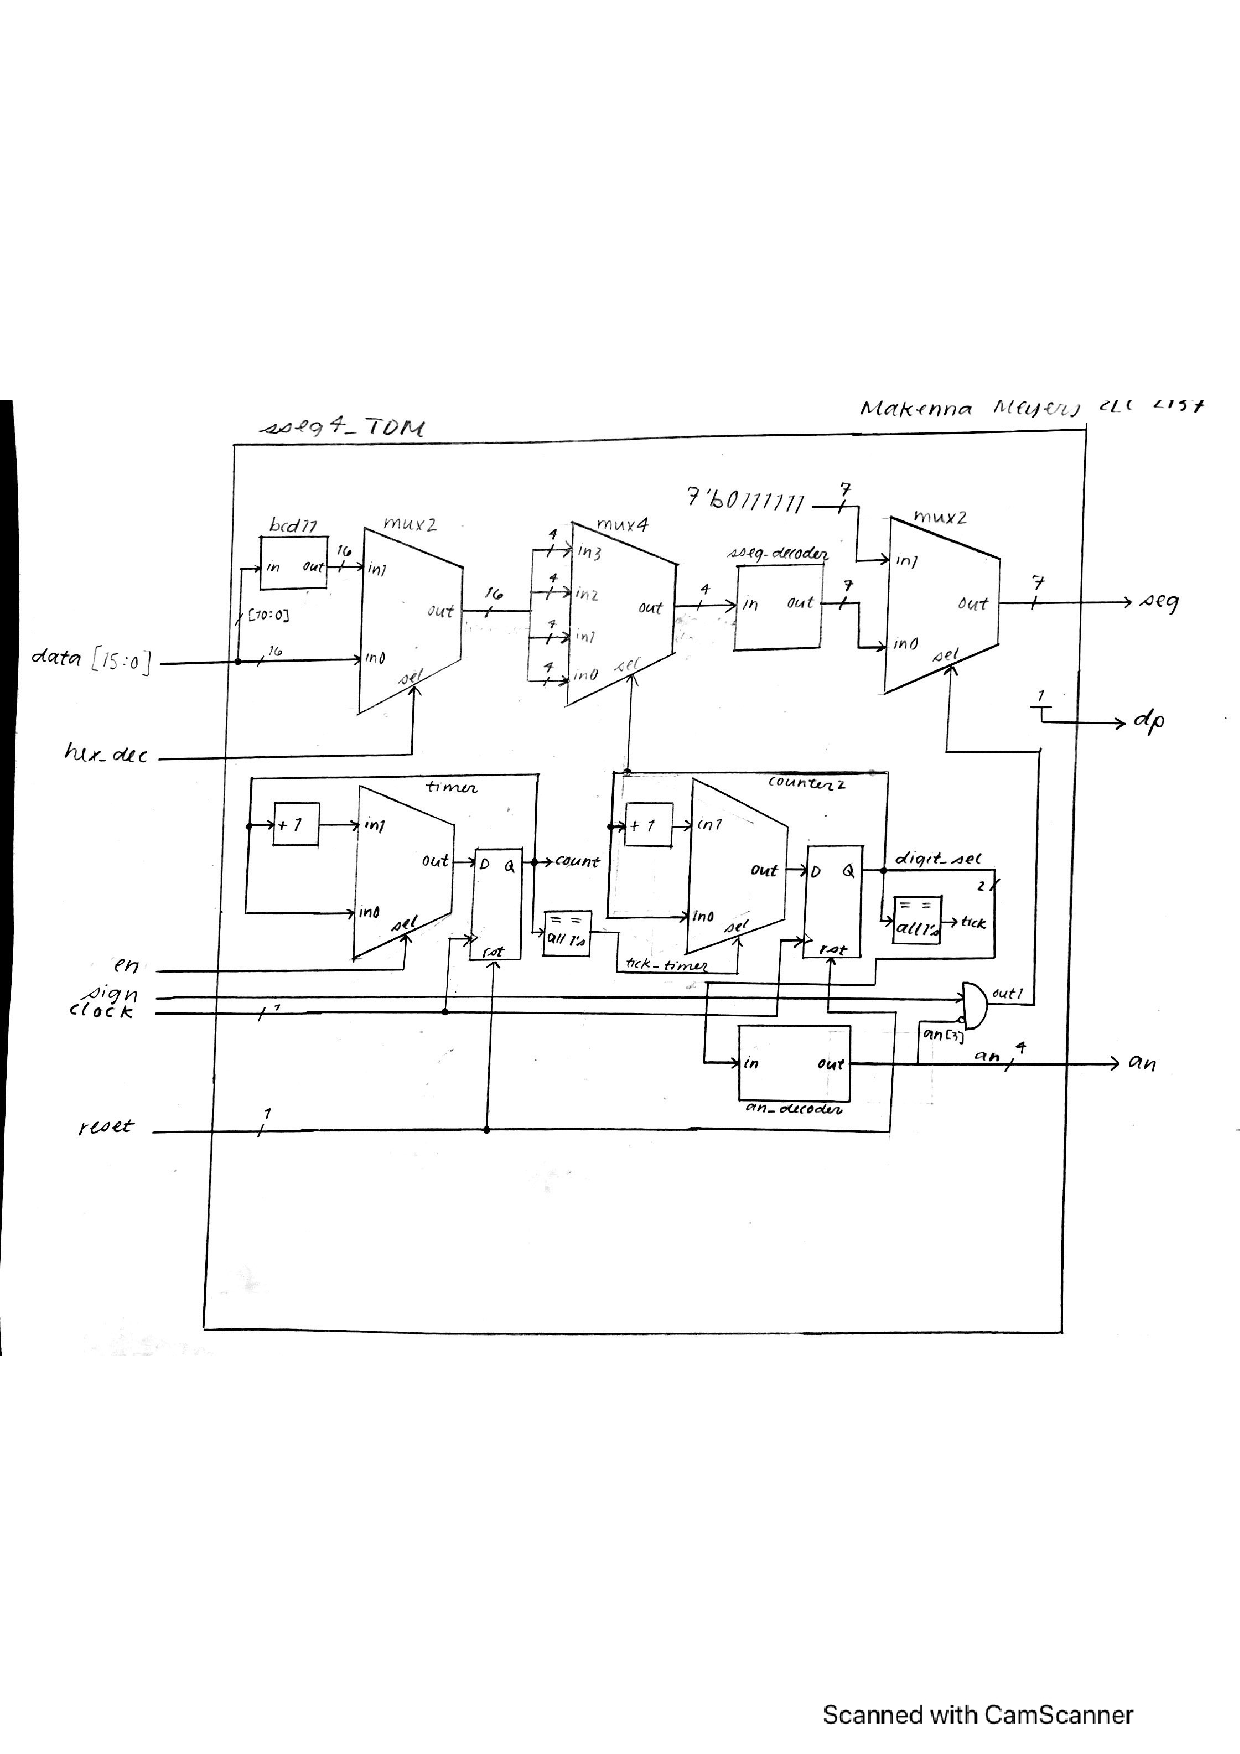
\includegraphics[width=0.8\textwidth,trim=0.5cm 6.5cm 1cm 7.08cm,clip]{sseg4_TDM_schematic}
	\caption{7-seg Driver Schematic}
	\label{fig:sseg4_TDM_schematic}			
\end{figure}
\clearpage

\begin{figure}[ht]\centering
	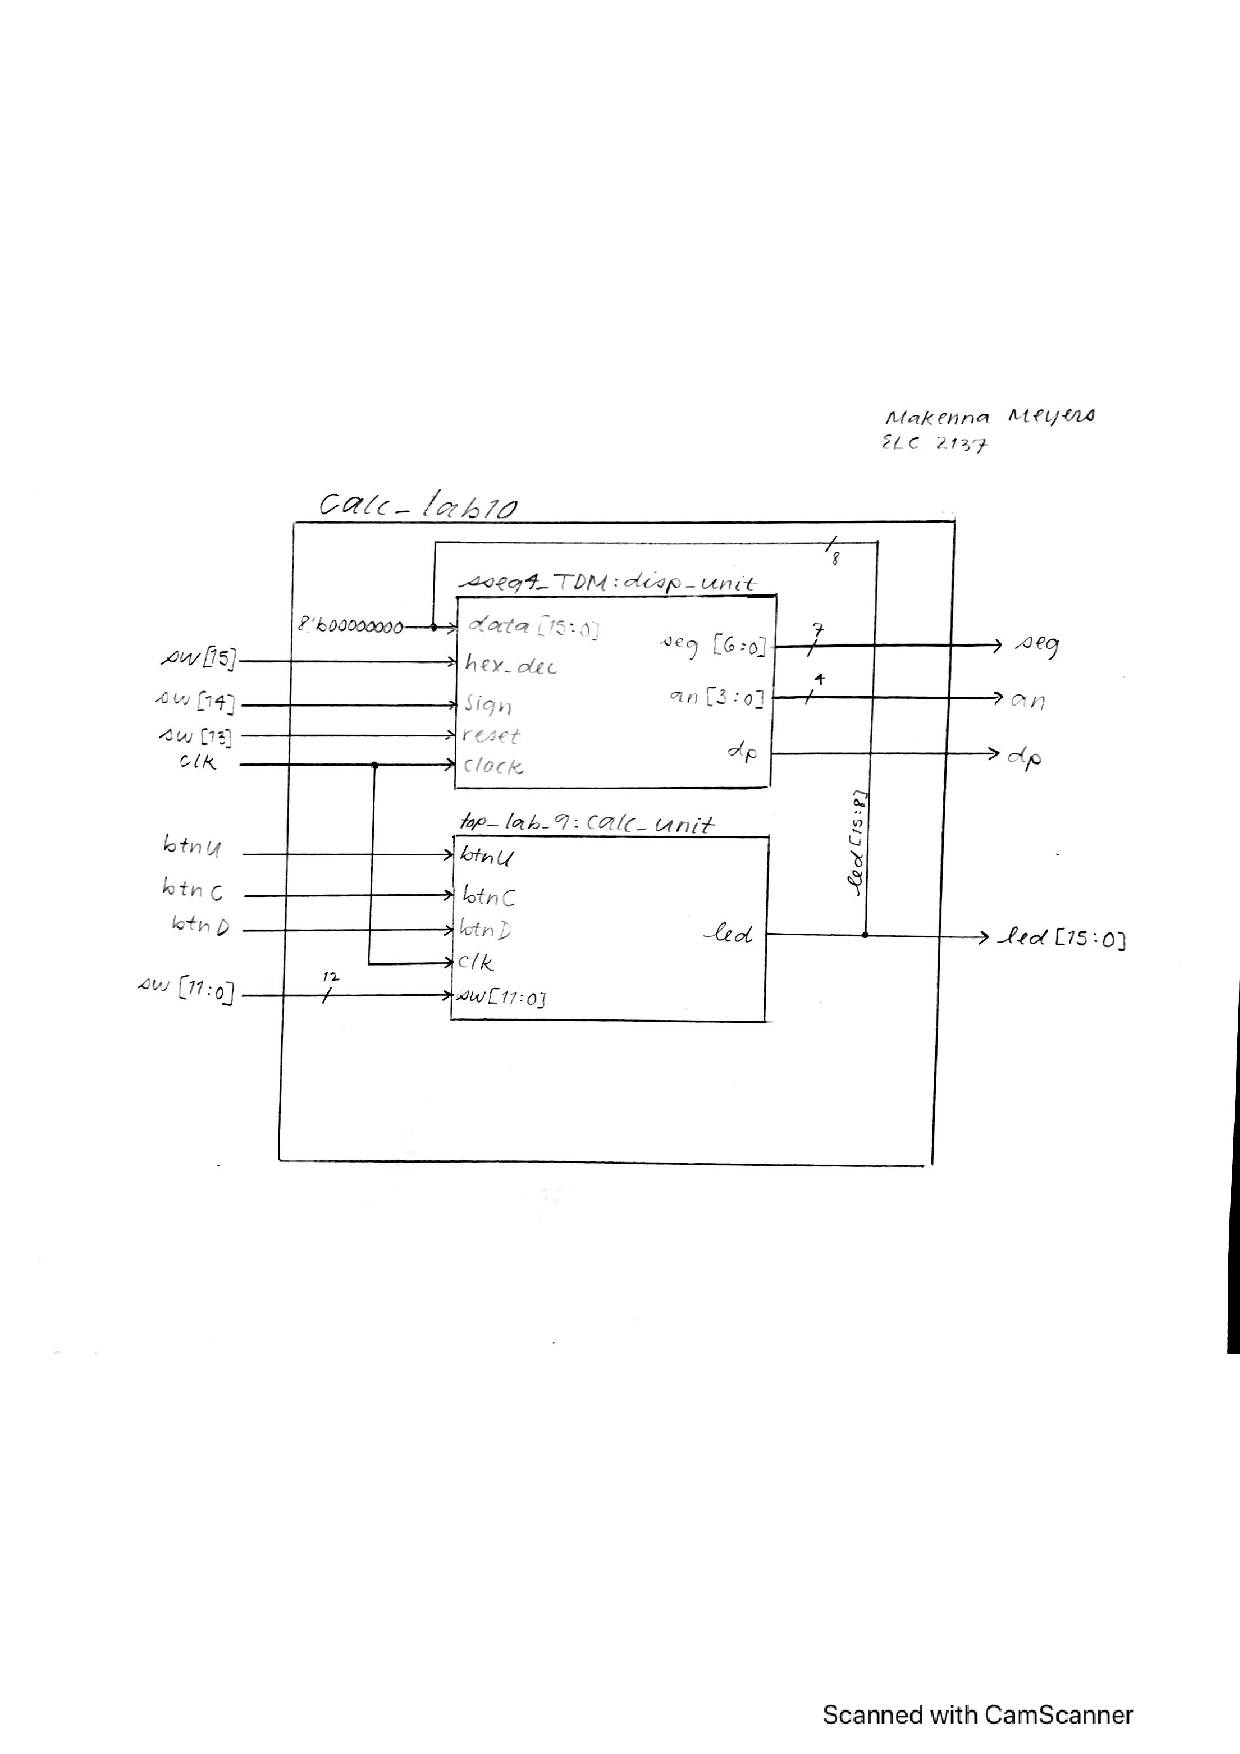
\includegraphics[width=0.8\textwidth,trim=2cm 9cm 3cm 8cm,clip]{calc_lab10_schematic}
	\caption{Calculator Schematic}
	\label{fig:calc_schematic}			
\end{figure}
\clearpage

			
\section*{Code}

\Verilog[caption=Counter Module,label=code:counter]{counter.sv}

\Verilog[caption=Counter Test Bench,label=code:counter_test]{counter_test.sv}

\Verilog[caption=7-seg Driver Module,label=code:sseg4_TDM]{sseg4_TDM.sv}

\Verilog[caption=7-seg Driver Test Bench,label=code:sseg4_TDM_test]{sseg4_TDM_test.sv}

\Verilog[caption=Calculator Module,label=code:calc_module]{calc_lab10.sv}

\end{document}